% Generated by scireport <version> (template generic@1, layout minimal@1) from a bundle with manifest sha256 7112702977a0. Do not edit.
\documentclass[11pt,a4paper]{article}
\usepackage{scireport-minimal}
\definecolor{accent}{HTML}{1F4E79}
\hypersetup{pdftitle={Full-kinds report},pdfcreator={scireport <version>}}
\begin{document}
\title{Full-kinds report \\[0.4em] \large Every v1.0 kind}
\author{N. Cardoso}
\date{2026-10-09 \\ Version 1.0.0 \\ compat corpus}
\maketitle

\begin{abstract}
A report that exercises \textbf{every} kind.
\end{abstract}
\tableofcontents

Short \textbf{markdown} text.

\section{Values}\label{a1}

\noindent\textbf{Number:} 1.23 \ensuremath{\pm} 0.01~arcsec\par

\begin{center}
\small
{\par\captionof{table}{A Parquet table}}
\begin{tabular}{>{\raggedleft\arraybackslash}p{\dimexpr 0.3333\linewidth-2\tabcolsep\relax}>{\raggedleft\arraybackslash}p{\dimexpr 0.3333\linewidth-2\tabcolsep\relax}>{\raggedright\arraybackslash}p{\dimexpr 0.3333\linewidth-2\tabcolsep\relax}}
\toprule
\textbf{ID} & \textbf{Redshift} & \textbf{label}\\
\midrule
1 & 0.100 & a\\
2 & -- & b\\
3 & 0.300 & c\\
\bottomrule
\end{tabular}
\end{center}

\begin{figure}[htbp]
\centering
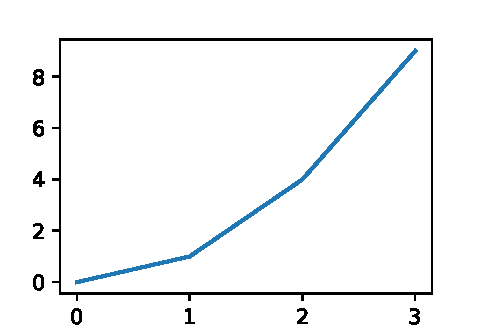
\includegraphics[width=0.6\linewidth]{figures/kinds.figure.pdf}
\caption{y = x squared}
% alt: A rising curve
\end{figure}

\end{document}
